\documentclass[
	a4paper,     		%% Papiergroesse: A4 OBSOLETE
%	twoside,     		%% Zweiseitiges Layout (alternativ: oneside)
	headsepline, 		%% Horizontale Linie unter Kopfzeile
	footsepline, 		%% Horizontale Linie ueber Fusszeile
	titlepage,   		%% Eigenstaendige Titelseite (alternativ: notitlepage)
%	halfparskip, 		%% Halbe Leerzeile zwischen zwei Abschnitten (alternativ: parskip, ...)
	12pt,        		%% Schriftgroesse: 12pt (alternativ: 10pt, 11pt, ...) OBSOLETE
%	bibtotoc,			%% Bilbiographie in's Inhaltsverzeichnis aufnehmen
	liststotoc,			%% Indexe in's Inhaltsverzeichnis aufnehmen
%	smallheadings,		%% Kleine Ueberschriften
%	DIV1,				%% Divisor, Zeilenlänge ca. 70 Zeichen
%	BCOR01cm,			%% Bindekorrektur
% 	draft			  	%% Entwurfsmodus, volle/leere Boxen markieren
%	abstracton			%% Titel "`Zusammenfassung"' einschalten
]{scrreprt}

%%%
%%% Pakete
%%%

%%% Literaturverzeichnis, deutschen Stil benutzen (dinat)
%%% TODO: funktioniert leider derzeit nicht mit TeXlipse!
%\usepackage[square]{natbib}
%\citestyle{dinat}

%%% Grafik
\usepackage{pstricks}

%%% Subfigures
\usepackage{subfig}

%%% Deutsche Sprache verwenden
\usepackage{ngerman}

%%% Kodierung der Eingabezeichen setzen (fuer dt. Umlaute etc.)
%%% Für Linux: [latin1] für Windows: [ansinew]
\usepackage[utf8]{inputenc}

%%% Zeichen-Kodierung in PDF-Dokumenten
\usepackage[T1]{fontenc}
%\usepackage{ae,aecompl}

%%% Web-Addressen auch mit T1-Encoding
\usepackage[T1]{url}
%%% ... und in tt-Font
\urlstyle{tt}

%%% amsmath, amssymb, amstext: Unterstuetzung div. mathematischer Zeichen etc.
\usepackage{amsmath,amssymb,amstext}

%%% pifont: "pifont Xs and Check Marks"
% \usepackage{pifont}

%%% PostScript-Fonts ersetzen
\usepackage{psfrag}

%%% Programmcode einbinden, Listings
\usepackage{listings}

%%% Farb-Unterstuetzung
\usepackage{color}

%%% Tabellen
\usepackage{booktabs}
\usepackage{array}
\usepackage{multirow}
\usepackage{tabularx}
\usepackage{threeparttable}	% Fussnoten in table-Umgebung

%%% Floats strikter positionieren (Option 'H'ere)
\usepackage{float}

%%%
%%% Pakete konfigurieren, Definitionen
%%%

%%% Ueberschriften bis zur Ebene 3 nummerieren
\setcounter{secnumdepth}{3}

% \setcounter{tocdepth}{3}

%%% Neue Spaltentypen definieren
\newcolumntype{N}{>{\bfseries\scriptsize}l}
\newcolumntype{T}{>{\ttfamily\small}l}
\newcolumntype{V}[1]{
	>{\bfseries\scriptsize\raggedright\hspace{0pt}}p{#1}
}

%%% Ein paar Farbdefinitionen (s. http://texnik.de/listings/listing0.pdf)
\definecolor{hellgelb}{rgb}{1,1,0.8}
\definecolor{hellgrau}{rgb}{0.95,0.95,0.95}
\definecolor{colKeys}{rgb}{0,0,1}
\definecolor{colIdentifier}{rgb}{0,0,0}
\definecolor{colComments}{rgb}{1,0,0}
\definecolor{colString}{rgb}{0,0.5,0}

%%% Konfiguration des listing-Paketes
\lstset{%
	float=hbp,%
	basicstyle=\ttfamily\small,%\footnotesize, %
	identifierstyle=\color{colIdentifier}, %
	stringstyle=\ttfamily,%
	keywordstyle=\color{colKeys}, %
	commentstyle=\rmfamily,%
	stringstyle=\color{colString}, %
% 	commentstyle=\color{colComments}, %
	columns=flexible, %
	tabsize=2, %
	frame=tb, %
	extendedchars=true, %
	showspaces=false, %
	showstringspaces=false, %
	numbers=left, %
	numberstyle=\tiny, %
	breaklines=true, %
	backgroundcolor=\color{hellgrau}, %
	breakautoindent=true, %
	captionpos=b%,
	aboveskip=\bigskipamount,%
	belowskip=\medskipamount,%
	escapeinside={(*}{*)}, %
	mathescape, %
	language=Matlab, %
}

%%% Benoetigte Sprachen laden
\lstloadlanguages{Matlab}

%%%
%%% Seitenlayout, Schriften
%%%

%%% scrpage2: KOMA Kopf- und Fusszeile
\usepackage[automark]{scrpage2}

%%% KOMA-Script: Optionen
% \KOMAoptions{fontsize=12pt}
% \KOMAoptions{paper=a4}

%%% EM unterstrichen darstellen
%\usepackage{ulem}

%%% Schrift fuer Captions verkleinern
\setkomafont{captionlabel}{\scriptsize}
\setkomafont{caption}{\usekomafont{captionlabel}}

\makeatletter
\renewcommand{\fps@figure}{htbp}
\renewcommand{\fps@table}{htbp}
\makeatother

%%% Schrift fuer Ueberschriften umstellen
%\setkomafont{sectioning}{\normalcolor\bfseries}

%%% Schriften fuer Titel- und Fusszeile umstellen
%\setkomafont{pagehead}{\normalfont\sffamily}
\setkomafont{pagenumber}{\normalfont\rmfamily\slshape}

%%% Unterstuetzung fuer Grafiken
\usepackage[dvips]{graphicx}
\DeclareGraphicsExtensions{.eps}
\graphicspath{{../images}}

%%% Hyperlinks in PS-Dokumenten, Optionen s.o.
\usepackage[%
  dvips,
  colorlinks=false,
  breaklinks=true,				%% Duerfen Links umbrochen werden? (true|false)
]{hyperref}

%%% Links im dvips-Mode auch umbrechen
\usepackage{breakurl}

%%%
%%% Layout der Titelseite
%%%

%%% Titelkopf, erscheint oberhalb des Titels
\titlehead{
	\begin{figure}[H]
		\centering
		
\includegraphics[width=\textwidth]{../images/htwg-logo}
	\end{figure}
}

%%%% Subject, erscheint oberhalb des Titels
\subject{Genetische Algorithmen, SS 07}

%%% Titel
\title{Traveling Salesman Problem}

%%% Publisher, hier: Verantwortlicher Prof.
\publishers{%
	\small
  Prof.\ Dr.\,Erben, Fakultät Informatik, HTWG Konstanz
}

%%%% Autor. Weitere Autoren mit \and{<Name>} hinzufuegen
\author{%
	André Erb
	\and{%
		Jan Tammen
	}%
}%

%%% Datum setzen
\date{\today}

%%% Rueckseite der Titelseite
\lowertitleback{%
	\footnotesize%
	Erstellt mit \LaTeXe\ unter Verwendung des \KOMAScript-Pakets.
}

%%%
%%% Header und Footer
%%%

\pagestyle{scrheadings}

%%% Kopfzeile in den Rand ragen lassen
%\setheadwidth{textwithmarginpar}

%%% Fusszeile in den Rand ragen lassen
%\setfootwidth{head}

%%% \automark[rechte Seite]{linke Seite}
%\automark[subsection]{section}

%% Header links -- section
%\ihead[]{\rightmark}

%% Header rechts -- chapter
%\ohead[]{\leftmark}

%% Header mittig -- leer
\chead[]{}

%% Footer mittig -- leer
\cfoot[]{}

%% Footer rechts -- Seitenzahl
\ofoot[]{\thepage}

%%% Footer links -- Titel der Arbeit
\ifoot[]{\footnotesize{Genetische Algorithmen SS 07}}

%%%
%%% Beginn Hauptdokument
%%%
\begin{document}

%%% Titelseite erstellen
\maketitle

%%% Inhaltsverzeichnis erstellen
%\newpage
\tableofcontents

%%%
%%% Beginn Inhalt
%%%
\chapter{Einleitung}
\section{The Mozart Programming System}
In der vorliegenden Ausarbeitung soll das "`Mozart Programming System"'
\footnote{\url{http://www.mozart-oz.org}} 
vorgestellt werden. Bei \textsl{Mozart} handelt es sich um eine 
Programmierumgebung, die die multiparadigmische Programmiersprache \textsl{Oz} 
implementiert.

Entstanden ist Mozart-Oz ursprünglich als Forschungsprojekt am Deutschen 
Forschungszentrum für Künstliche Intelligenz (DFKI) sowie der Universität 
Saarbrücken. Inzwischen wird die Sprache vom Mozart-Konsortium, zu welchem 
Arbeitsgruppen aus Belgien, Schweden und Deutschland gehören, weiterentwickelt. 
Die Quellen sind unter einer Open-Source-Lizenz verfügbar; ein kommerzieller 
Einsatz der Sprache ist ebenfalls möglich.

Ähnlich wie in Java können Oz-Programme in eine Art Byte-Code übersetzt werden 
und laufen anschließend in einer virtuellen Maschine ab. Auf diese Weise wird 
eine gewisse Plattformunabhängigkeit erreicht.

\section{Die Programmiersprache Oz}
\subsection{Features}
Als Hauptfeatures und -vorteile von Oz gelten die folgenden Aspekte:

\begin{description}
  \item[Nebenläufigkeit] Arbeit mit leichtgewichtigen Threads, 
  Datenfluss-Synchronisation.
  \item[Inferencing] Constraintbasierte und 
  logische Programmierung.
  \item[Verteilung] Transparente 
  Netzwerkunterstützung.
  \item[Flexibilität] Dynamische Typisierung, inkrementelles 
  Kompilieren.
\end{description}

\subsection{Datentypen}
Die Sprache stellt eine Reihe von Datentypen zur Verfügung, deren Hierarchie in 
Abbildung \ref{fig:oz-datentypen} dargestellt ist.

\begin{figure}[hp]
  \centering 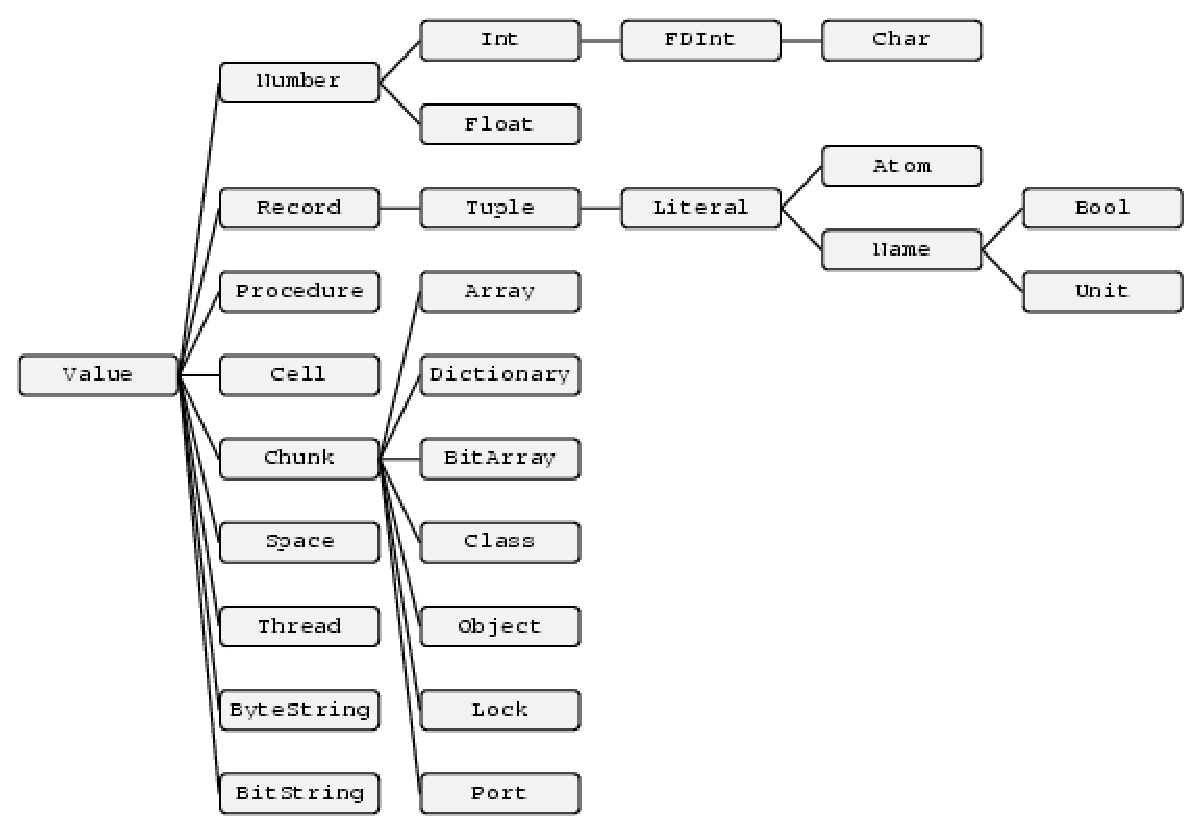
\includegraphics[width=0.70\textwidth]{../images/oz-datentypen} 
  \caption{Hierarchie der Datentypen in Oz 3. Quelle:
  \cite[Tutorial of Oz, Chapter 3.1]{url:mozart-documentation}}
  \label{fig:oz-datentypen}
\end{figure}

Einige der wichtigsten Datentypen seien hier kurz aufgeführt (vgl. 
\cite{Brunklaus:00}).

\begin{enumerate}
  \item Einfache Werte
    \begin{description}
      \item [Zahlen] können in Oz sowohl als ganze Zahlen (\texttt{Int, Char})
      als auch Fließkommazahlen (\texttt{Float}) benutzt werden.
      \item[Literale] teilen sich auf in sog. Atome und Namen. Ein Atom wird 
      durch eine alphanumerische Zeichenkette beschrieben, die entweder mit 
      einem Kleinbuchstaben beginnt oder in Hochkomma gefasst ist. Namen sind 
      eindeutige Bezeichner, die über eine spezielle Prozedur namens 
      \texttt{NewName} erzeugt werden können.
      \item[Prozeduren] können in Oz an Variablen gebunden und auch zur 
      Laufzeit erzeugt werden. \end{description}
  \item Zusammengesetzte Werte
    \begin{description}
      \item[Records] bestehen aus einem Bezeichner (Label) sowie einer festen 
      Anzahl von Komponenten oder Argumenten. Argumente bestehen aus dem Tupel 
      (Feature, Feld).
      \item[Tupel] sind ein Spezialfall von Records, bei denen die Argumente 
      kein explizites Feature besitzen.
      \item[Listen] sind eine Sonderform der Tupel. Die leere Liste wird mit
      \texttt{nil} denotiert, offene Listen bspw. als \texttt{1|2|3|nil} und 
      geschlossene Listen (also Listen mit fester Elementanzahl) als \texttt{[1 
      2 3]}.
    \end{description}
  \item \textbf{Chunks} erlauben es, abstrakte Datentypen zu konstruieren. 
  Oz bringt bereits einige vordefinierte Chunks mit, z.B. \texttt{Array} 
  oder \texttt{Dictionary}.
\end{enumerate}

\subsection{Multiparadigmisch?}
Wie bereits eingangs erwähnt, unterstützt Oz mehrere Programmierparadigmen:

\begin{enumerate}
  \item Constraint-Programmierung
  \item Funktionale Programmierung
  \item Objektorientierte Programmierung
  \item Logische Programmierung
\end{enumerate}
  
Im Gegensatz zu einer Programmiersprache, die nur eines der Paradigmen 
unterstützt, lassen sich in Oz also die zu lösenden Probleme von mehreren 
Seiten gleichzeitig mit dem jeweils geeignetsten Paradigma bearbeiten. 
Erreichen könnte man dies zwar auch durch die Kombination verschiedener 
Programmiersprachen, dabei bliebe aber der Nachteil, dass man semantische 
Lücken überwinden und Schnittstellen zwischen den einzelnen Sprachen definieren 
müsste. Dies würde u.a. zu einer aufwendigeren Fehlersuche führen. Mit Oz 
lassen sich hingegen die verschiedene Paradigmen problemlos miteinander 
kombinieren, deren gemeinsame Basis, das Oz Programming Model, im nächsten 
Abschnitt vorgestellt wird.

\subsection{Programmiermodell (Oz Programming Model, OPM)}
Die Grundlage für Berechnungen in Oz bildet das so genannte \textsl{Concurrent 
Constraint Programming}. Alle weiteren Paradigmen werden durch sog. "`syntactic 
sugar"' (Syntaxerweiterungen) in die Sprache integriert \cite{KI-LP96}.

Allgemein verwendet das Modell für Berechnungen die Metapher eines sog. 
\textsl{Berechnungsraums} (Computational Space). In diesem befindet sich zum 
einen ein \textsl{Speicher}, zum anderen eine Anzahl von sog. \textsl{Aktoren}. 
Aktoren führen die eigentlich Berechnung durch, indem sie schrittweise 
reduziert werden und sich dabei über den gemeinsamen Speicher synchronisieren. 
Dazu können Aktoren Information in den Speicher schreiben (tell) und auf 
Information warten und diese anfordern (ask).

Nebenläufigkeit (Concurrency) ist einer der wichtigsten Aspekte des OPM. Dabei 
bedeutet Nebenläufigkeit, dass verschiedene Berechnungen unabhängig voneinander 
durchgeführt werden können, nicht, dass diese parallel ablaufen.


\chapter{Aufgaben}
\section{Aufgabe a}
Nach Durchführung einiger Testläufe mit dem Demoskript \texttt{demotsplib.m} 
und dem TSP-Problem \texttt{bays29.tsp} zeigte sich, dass die Ergebnisse i.A. 
noch recht weit vom Optimalwert 2020 (vgl. \cite[Appendix]{Reinelt94}) entfernt 
waren.

Das Beispielskript ist standardmäßig mit den folgenden Parametern konfiguriert:

\begin{itemize}
  \item \texttt{NumberSubpopulation}: Anzahl der Subpopulationen, 6
  \item \texttt{NumberIndividuals}: Anzahl der Individuen pro Population, 50
  \item \texttt{Selection.GenerationGap}: Anzahl der Individuen pro Population, 0.95
  \item \texttt{Termination.Method}: Art des Abbruchkriteriums, 1 (entspricht
  dem Erreichen der maximalen Anzahl von Generationen)
  \item \texttt{Termination.MaxGen}: Anzahl der Generationen, nach denen der
  Algorithmus terminieren soll, 400
\end{itemize}

Durch die Wahl des genetischen Algorithmus' \texttt{tbx3perm} sind implizit 
weiterhin die folgenden Einstellungen gegeben:

\begin{itemize}
  \item \texttt{VariableFormat}: Format der Variablen und Konvertierung 
  zwischen diesem und in dem intern verwendeten Format, 5 (entspricht einem 
  nicht festgelegten Format, demzufolge findet auch keine Konvertierung statt).
  \item \texttt{Recombination.Name}: Verwendetes Rekombinationsverfahren, 
  \texttt{recpm} (entspricht Partial Matching Recombination)
  \item \texttt{Mutation.Name}: Verwendetes Mutationsverfahren, \texttt{mutswap}
  (entspricht Swap Mutation)
\end{itemize}

\section{Aufgabe b}
\subsection{Architektur des Testsystems}
\label{subsec:ArchitekturTestsystem}
Für die Durchführung der Tests wurde zunächst das der GEATbx beiliegende Skript
\textbf{demotsplib.m} als Ausgangsbasis benutzt. Alle für die Testläufe zu
variierenden Parameter lassen sich im Kopf des Skriptes \textbf{tsp.m} in
Variablenform festlegen. 

Für die Durchführung der Aufgabe c) waren beispielsweise die Anzahl der
Subpopulationen und der Individuen pro Population in verschiedenen
Konstellationen zu testen. Zusätzlich dazu lassen wir für jede
Variablenkombination eine definierbare Anzahl von Testläufen laufen, um später
Mittelwert und Standardabweichung berechnen zu können. Listing
\ref{lst:testsystem-pseudo} zeigt den beispielhaften Aufbau des Testskripts für
Aufgabe c). Für Aufgabe d) wurde eine modifizierte Version des in
\ref{lst:testsystem-pseudo} beschriebenen Skriptes eingesetzt. Der Pseudocode
zu der genannten Modifikation wird in Listing \ref{lst:testsystemTeilD}
aufgeführt. Der komplette Code der Skripte \ref{lst:testsystem-pseudo} und
\ref{lst:testsystemTeilD} ist im Anhang aufgeführt.

\begin{lstlisting}[language=Pseudo, label={lst:testsystem-pseudo}, 
caption={Pseudocode Testskript Teil B}]
Subpopulationen = (1, 5, 8, 12)
Individuen = (15, 30, 45, 60)
AnzahlTestlaeufe = 20

foreach anzahlSubpopulationen in Subpopulationen do
	foreach anzahlIndividuen in Individuen do
		for <AnzahlTestlaeufe> do
			Fuehre genetischen Algorithmus aus
			Berechne Minimal-/Maximalwert
		end for
		Ergebnisausgabe Logfile
	end foreach
end foreach
\end{lstlisting}

\begin{lstlisting}[language=Pseudo, label={lst:testsystemTeilD}, 
caption={Pseudocode Testskript Teil D}]
Subpopulationen  = 12;
Individuen 	     = 60;
AnzahlTestlaeufe = 20;

SelektionsMethoden = (selsus, selrws, seltour)

foreach SelektionsMethode in SelektionsMethoden do
	for <AnzahlTestlaeufe> do
			Fuehre genetischen Algorithmus aus
			Berechne Minimal-/Maximalwert
	end for
		Ergebnisausgabe Logfile
end foreach
\end{lstlisting}

Zur späteren Auswertung der Ergebnisse werden alle relevanten Daten in ein
Logfile protokolliert. Abbruchkriterium für die genetische Optimierung ist hier
das Erreichen der Maximalgeneration 100.

\subsubsection{Eingesetzte Hard- und Software}
Die Tests der Aufgabe c) wurden auf einem Pentium M mit 1.6 GHz unter 
Verwendung von Matlab 5.3 und GEATbx Version 3.8 durchgeführt.

\section{Aufgabe c}
\subsection{Migration}
Bei der Verwendung mehrerer Subpopulationen entwickeln sich diese zunächst 
unabhängig voneinander. Um nun aber auch global von den lokal in den 
Subpopulationen entstandenen Individuen profitieren zu können, wird nach 
einiger Zeit Information zwischen den einzelnen Populationen ausgetauscht - 
dies geschieht durch den Austausch einzelner Individuen. Diesen Vorgang nennt 
man \textsl{Migration}. Nach dem Austausch von Individuen entwickeln sich die 
Populationen wieder eine Zeit lang unabhängig voneinander, bis der 
Austauschvorgang von neuem beginnt \cite{url:geatbx-documentation}.

Der Parameter \texttt{Topology} legt fest, welche Topologie bei der Migration 
verwendet wird. Unter Topologie ist in diesem Zusammenhang zu verstehen, 
\textsl{welche} Unterpopulationen Individuen untereinander austauschen. Dieser 
Parameter kann in der GEATbx die folgenden drei Werte annehmen:

\begin{itemize}
  \item 0: Vollständige Netzstruktur ohne Einschränkungen, d.h. Individuen 
  können zwischen \textsl{allen} Subopulationen ausgetauscht werden.
  \item 2: Ringstruktur, d.h. die Subpopulationen werden ringförmig angeordnet 
  und Individuen können nur in die im Ring folgende Subpopulation migrieren.
  \item 1: Nachbarschaftsstruktur, ähnlich zur Ringstruktur. Jedoch können 
  Individuen in beiden Richtungen zwischen den Nachbarn transferiert werden.
\end{itemize}

Der Parameter \texttt{Rate} bestimmt, welcher Anteil jeder Population bei der 
Migration migriert werden soll. Dabei können Werte im Bereich von $[0, 1]$ 
angegeben werden. Die Werte repräsentieren prozentuale Angaben; so sorgt also 
z.B. das Setzen des Parameters auf den Wert 0.20 dafür, dass 20\% der 
Individuen bei der Migration ausgetauscht werden. Mittels des Parameters 
\texttt{Interval} lässt sich einstellen, wie oft (d.h. nach welcher Anzahl von 
Generationen) eine Migration stattfinden soll.

\subsection{Testläufe mit variierenden Populationsgrößen}
\label{subsec:TestlaeufePopulationsgroessen}
Für die Durchführung dieser Testreihe wurde das bereits beschriebene Skript 
verwendet; variiert wurden die folgenden Parameter:

\begin{description}
  \item[Subpopulationen:] 1, 5, 8 und 12.
  \item[Individuen pro Population:] 15, 30, 45, 60.
\end{description}

Für die 16 möglichen Kombinationen wurden jeweils 20 Testläufe durchgeführt und
am Ende der Mittelwert berechnet. Insgesamt umfasste die Testreihe demnach 320
Testläufe. Die Anzahl der Generationen war hierbei stets auf 100 fixiert.

Die Ergebnisse der Testläufe sind in Tabelle \ref{tbl:aufgabeC-ergebnisse}
aufgeführt. 

\begin{table}
	\sffamily
	\centering
	\footnotesize
	\begin{tabularx}{\textwidth}{NXlllll}
		\toprule
		\multicolumn{1}{@{}N}{Nr.} &
		\multicolumn{1}{V{3.5em}@{}}{Subpop.} &
		\multicolumn{1}{V{3.5em}@{}}{Indiv.} &
		\multicolumn{1}{V{5em}@{}}{Mittelwert $\bar{x}$} &
		\multicolumn{1}{V{6.5em}@{}}{Standardabw. $\sigma_x$} &
		\multicolumn{1}{V{9em}@{}}{Minimalwert in Lauf $r$, Generation $g$} &
		\multicolumn{1}{V{9em}@{}}{Maximalwert in Lauf $r$, Generation $g$} \\
		\midrule\addlinespace
		1 & 1 & 15 & 3093,30 & 215,63 & 2793, $r = 10$, $g = 95$ & 3715, $r = 20$, $g
		= 95$ \\ \cmidrule(rl){1-7}
		2 & 5 & 15 & 2693,55 & 128,33 & 2443, $r = 12$, $g = 97$ & 2889, $r = 11$, $g
		= 94$ \\ \cmidrule(lr){1-7}
		3 & 8 & 15 & 2644,65 & 136,63 & 2361, $r = 15$, $g = 94$ & 2904, $r = 16$, $g = 99$ \\ \cmidrule(lr){1-7}
		4 & 12 & 15 & 2521,25 & 91,48 & 2269, $r = 16$, $g = 91$ & 2662, $r = 14$, $g = 97$ \\
		\midrule
		5 & 1 & 30 & 3024,40 & 243,43 & 2719, $r = 5$, $g = 89$ & 3567, $r = 18$, $g = 100$ \\ \cmidrule(lr){1-7}
		6 & 5 & 30 & 2464,70 & 119,89 & 2253, $r = 2$, $g = 88$ & 2857, $r = 7$, $g = 97$ \\ \cmidrule(lr){1-7}
		7 & 8 & 30 & 2448,15 & 112,17 & 2192, $r = 3$, $g = 99$ & 2622, $r = 7$, $g = 87$ \\ \cmidrule(lr){1-7}
		8 & 12 & 30 & 2416,70 & 103,81 & 2209, $r = 5$, $g = 96$ & 2564, $r = 9$, $g = 95$ \\
		\midrule
		9 & 1 & 45 & 2838,25 & 213,74 & 2493, $r = 6$, $g = 91$ & 3153, $r = 17$, $g = 83$ \\ \cmidrule(lr){1-7}
		10 & 5 & 45 & 2378,00 & 117,79 & 2173, $r = 15$, $g = 100$ & 2632, $r = 3$, $g = 99$ \\ \cmidrule(lr){1-7}
		11 & 8 & 45 & 2347,50 & 105,99 & 2189, $r = 11$, $g = 99$ & 2610, $r = 14$, $g = 96$ \\ \cmidrule(lr){1-7}
		12 & 12 & 45 & 2309,85 & 98,98 & 2168, $r = 9$, $g = 99$ & 2497, $r = 17$, $g = 90$ \\
		\midrule
		13 & 1 & 60 & 2747,60 & 157,29 & 2395, $r = 16$, $g = 100$ & 3071, $r = 8$, $g = 99$ \\ \cmidrule(lr){1-7}
		14 & 5 & 60 & 2386,35 & 101,48 & 2157, $r = 19$, $g = 96$ & 2558, $r = 8$, $g = 98$ \\ \cmidrule(lr){1-7}
		15 & 8 & 60 & 2320,75 & 105,88 & 2143, $r = 4$, $g = 97$ & 2540, $r = 18$, $g = 99$ \\ \cmidrule(lr){1-7}
		16 & 12 & 60 & \textbf{2285,85} & 88,91 & \textbf{2115}, $r = 20$, $g = 90$ & 2422, $r = 8$, $g = 96$ \\

		\addlinespace\bottomrule
		\end{tabularx}
	\caption{Ergebnisse der Testreihe}
	\label{tbl:aufgabeC-ergebnisse}
\end{table}

\subsubsection{Interpretation der Ergebnisse}
Wie man an den Testergebnissen sieht, erhöht sich die Güte des Resultats sowohl
mit der Anzahl der \textsl{Subpopulationen} als auch der \textsl{Individuen pro
Population}. Innerhalb der Testläufe mit gleicher Individuenanzahl verbessert
sich der Mittelwert deutlich mit steigender Subpopulationsanzahl. Und auch
zwischen den Testfällen mit steigender Individuenanzahl ist erkennbar, dass die
Ergebnismittelwerte besser sind. Abbildung \ref{fig:aufgabeC-plot} zeigt eine
grafische Auswertung der Testergebnisse.

\begin{figure}
  \centering
  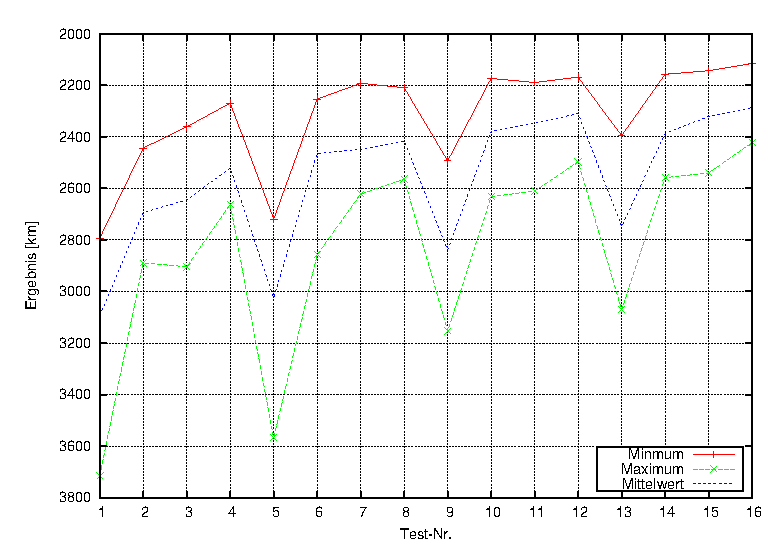
\includegraphics[width=1.0\textwidth]{../images/aufgabeC-plot}
  \caption{Grafische Darstellung der Testreihe: Minimal-, Maximal- und
  Mittelwert}
  \label{fig:aufgabeC-plot}
\end{figure}

Das beste Testergebnis von 2115 km (in der Tabelle fett markiert) erhielten wir
erwartungsgemäß bei den jeweiligen Maximalwerten der variierten Parameter.

\section{Aufgabe d}
\subsection{Roulette Wheel und Stochastic Universal Sampling}
Bei dem von 'geatbx' angebotenem Verfahren 'selsus' handelt es sich um das
'Stochastic Universal Sampling'. Sowohl das 'selsus' wie auch das 'Roulette
Wheel'-Verfahren, dienen nach \cite{url:geatbx-documentation}
zur Auswahl der Paarungs-Populationen. Dabei erhalten die zu auszuwählenden
Individuen einen Bereich zugeteilt, der in seiner Größe relativ zum 
Fitnesswert und somit auch zur Auswahlwahrscheinlichkeit eines Individuums
steht. Beide Verfahren suchen nun per Zufall positionierter Zeiger, die
gewünschte Anzahl an Individuen aus. Der Unterschied zwischen dem 'Roulette-Wheel'
und dem 'selsus'-Verfahren besteht nun im Ziehungszeitpunkt. Während beim
'Roulette-Wheel'-Verfahren jedes Individuum in einem eigenen Durchlauf unabhängig
von den anderen gezogen wird, werden beim 'Stochastic Universal Sampling' alle
Individuen auf einmal gezogen. Durch diese Vorgehensweise sind die 
Auswahl-Wahrscheinlichkeiten voneinander, und damit von der jeweiligen Ziehung
abhängig, da es sich um Ziehen ohne Zurücklegen handelt.

Abbildung \ref{fig:RouletteSelsus} nach \cite{url:RouletteSelsus} verdeutlicht 
die oben beschriebenen Aspekte.
Es werden pro Selektionsverfahren je 4 Individuen, $Q_1$ bis $Q_4$ ausgewählt.
Beim 'Roulette-Wheel'-Verfahren finden dabei 4 Ziehungen statt, während beim
'selsus'-Verfahren 1 Ziehung durchgeführt wird.  

\begin{figure} 
  \centering
  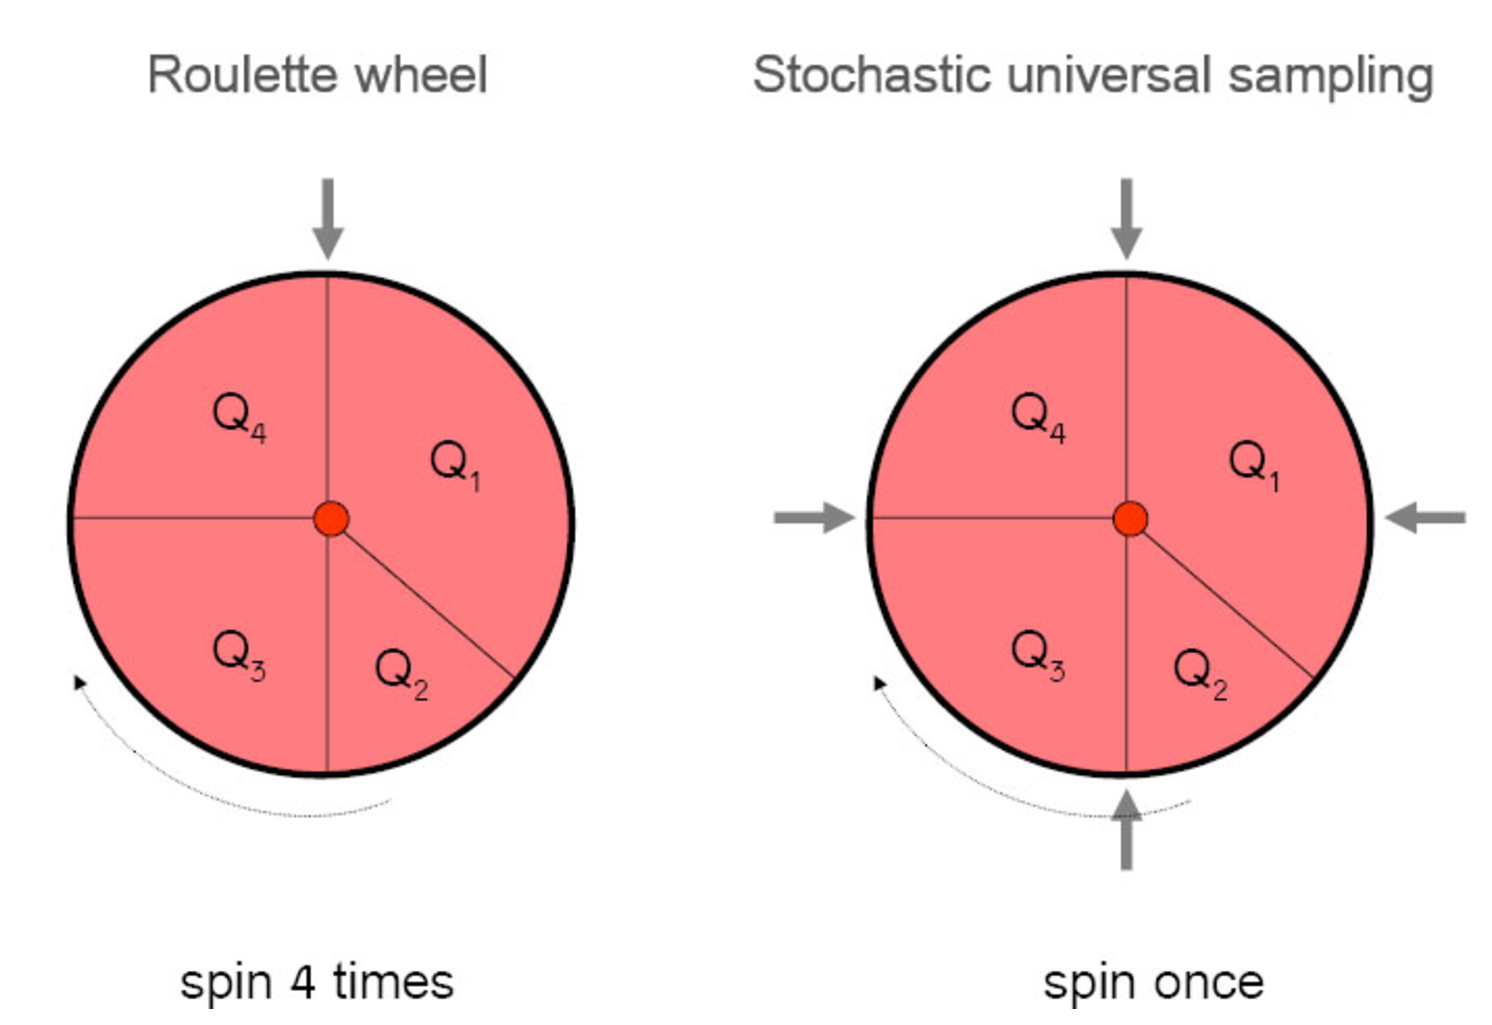
\includegraphics[width=0.6\textwidth]{../images/picRouletteSelsus}
  \caption{Selektionsverf. 'Roulette-Wheel' und 'Stochastic Universal Sampling'.}
  \label{fig:RouletteSelsus}
\end{figure}

Nachfolgende Abbildung nach \cite{url:geatbx-documentation} zeigt die von
\cite{url:geatbx-documentation} beschriebene Implementierung von 'selsus'.
Dabei werden die Zeiger, welche die Indiv. auswählen im gleichen Abstand
$1/n$ angeordnet sind. $n$ bezeichnet dabei die Anzahl der auszuwählenden
Individuen. Die Zufallszahl entscheidet nun über den Anfangspunkt der 
Zeigeranordnung, welche alle Individuen gleichzeitig wählt. In der Ziehung
des zeigten Beispiels nach \cite{url:geatbx-documentation}, ergeben sich 
hierdurch die Individuen 1, 2, 3, 4, 6, 8.
       
\begin{figure} 
  \centering
  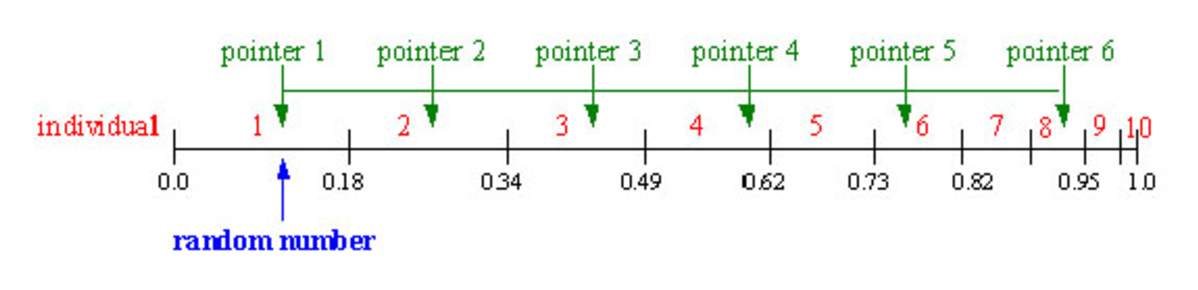
\includegraphics[width=0.8\textwidth]{../images/picSelsusAuswahl}
  \caption{Beispielziehung mit Hilfe des 'Stochastic Universal Sampling'.}
  \label{fig:SelsusAuswahl}
\end{figure}

\subsection{'Tournament'-Selektion}
Bei der 'Tournament'-Selektion lässt man nach \cite{url:geatbx-documentation}
zufällig ausgewählte Individuen gegeneinander antreten. Der jeweils fitteste
der 'Tournament'-Gruppe wird schließlich selektiert. Dieser Vorgang wird so
oft wiederholt, bis die gewünschte Anzahl an zu selektierenden Individuen
erreicht ist.

Folgende Abbildung nach \cite{url:RouletteSelsus} verdeutlicht dies.
Dabei werden aus einer Subpopulation zufällig drei Indiv. ausgewählt, die
gegeneinander antreten. Das Individuum mit dem höchsten Fitnesswert (hier $7$),
wird schließlich in den 'Mating-Pool' aufgenommen.

\begin{figure} 
  \centering
  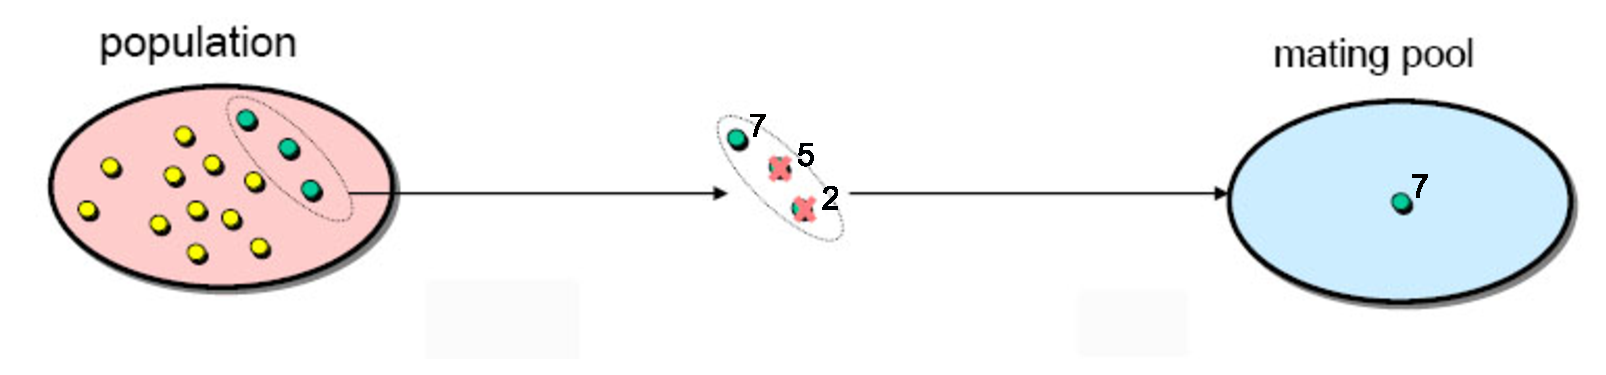
\includegraphics[width=0.8\textwidth]{../images/picTournamentAuswahl}
  \caption{Ziehung mit Hilfe der 'Tournament'-Selektion}
  \label{fig:TournamentAuswahl}
\end{figure}

\subsection{Testläufe mit variierenden Selektions-Methoden}
\label{subsec:TestlaufeSelektionsmethoden}
Für die Durchführung der Testreihen in Aufgabe d), wurde die in 
\ref{subsec:ArchitekturTestsystem} beschriebene Modifikation des
Testskriptes benutzt. 

\begin{description}
  \item[Selektions-Methoden:] selsus, selrws, seltour
\end{description}

Für jeden der 3 Selektionsarten wurden 20 Testläufe gefahren, womit 
sich eine Gesamtgröße von 60 Testläufen ergibt. Die in Aufgabe c) bereits durchgeführte
Testreihe von 12 Subpopulationen, 60 Individuen und der Selektionsart 'selsus',
wurde wiederholt. Die Ergebnisse ähneln dabei den in Tabelle 
\ref{tbl:aufgabeC-ergebnisse}
gezeigten Werten. So beträgt der Mittelwert aller wiederholten Testläufe
$2225.70$, während er in Aufgabe c) bei $2285.85$ lag. Vergleiche hierzu die
Ergebnisse aus Tabelle \ref{tbl:aufgabeD-ergebnisse}, der Zeile 1, mit den
Ergebnissen aus Tabelle \ref{tbl:aufgabeC-ergebnisse}, Testlauf Nr. 16.
Die vollständigen Testläufe, zu allen Selektionsarten, sind dem Anhang in Form
der entsprechenden Logging-Dateien zu entnehmen. 

\begin{table}
	\sffamily
	\centering
	\footnotesize
	\begin{tabularx}{\textwidth}{NXlllll}
		\toprule
		\multicolumn{1}{@{}N}{Selektion} &
		\multicolumn{1}{V{3.5em}@{}}{Subpop.} &
		\multicolumn{1}{V{3.5em}@{}}{Indiv.} &
		\multicolumn{1}{V{5em}@{}}{Mittelwert $\bar{x}$} &
		\multicolumn{1}{V{6.5em}@{}}{Standardabw. $\sigma_x$} &
		\multicolumn{1}{V{9em}@{}}{Minimalwert in Lauf $r$, Generation $g$} &
		\multicolumn{1}{V{9em}@{}}{Maximalwert in Lauf $r$, Generation $g$} \\
		\midrule\addlinespace
		
		selsus & 12 & 60 & 2225.70 & 119.76 & \textbf{2028}, $r = 1$, $g = 92$ & 2445, $r = 7$, $g = 100$ \\ \cmidrule(lr){1-7}
		selrws & 12 & 60 & 2234.45 & 113.72 & 2090, $r = 5$, $g = 99$ & 2479, $r = 18$, $g = 100$ \\ \cmidrule(lr){1-7}
		seltour & 12 & 60 & \textbf{2163.90} & 96.21 & 2036, $r = 1$, $g = 93$ & 2422, $r = 16$, $g = 94$ \\

		\addlinespace\bottomrule
		\end{tabularx}
	\caption{Ergebnisse aus 60 Testläufen, mit den Selektionsverfahren 'selsus', 'selrws' und 'seltour'.}
	\label{tbl:aufgabeD-ergebnisse}
\end{table}
 
\subsubsection{Interpretation der Ergebnisse}
Die Wiederholungstestläufe, die mit Hilfe der Selektionsart 'selsus' erzielt
wurden, ähneln  den Ergebnissen aus Kapitel \ref{subsec:TestlaeufePopulationsgroessen}.
Mit $2225.70$, konnte sogar ein leicht verbesserter Mittelwert erzielt werden. Allerdings
weichen dabei die einzelnen Werte mit einer Standardabweichung von $119.76$ km,
auch mehr vom Mittelwert ab, als in den Testläufen der Aufgabe c). Bei fest
vorgegebenen Parameterwerten von 12 Subpopulationen und 60 Individuen, liefert
das 'Roulette-Wheel'-Selektionsverfahren leicht schlechtere Ergebnisse als mit den
ersten 20 Testläufen des 'selsus'-Selektionsverfahrens. Das beste Ergebnis
lieferte die 'selsus'-Selektion mit einem minimalen Wert von 2028 Kilometern.
Im Mittel aller Werte lieferte jedoch die 'Tournament'-Selektion, mit $2163.90$ Kilometern
den besten Wert. Die einzelnen Werte zeigen dabei mit einer Standardabweichung von $96.21$ km,
eine verhältnismäßig geringe Streuung um den Mittelwert. Das schlechteste Ergebnis der
Selektionsart 'seltour', liegt mit $2422$ ebenfalls jeweils unter den Maximalwerten
der beiden ersten Selektionsarten, wie in Tabelle \ref{tbl:aufgabeD-ergebnisse}
gezeigt.
  
Somit konnte durch Ersetzen der Selektionsart 'selsus' durch das
'Roulette-Wheel'-Verfahren, keine signifikante Änderung der Ergebnisse erzielt
werden. Der Minimal- sowie der Mittelwert erreichten ein leicht schlechteres
Gesamtergebnis, welches keine genaueren Rückschlüsse zulässt. Durch Verwenden der 
'Tournament'-Selektionsart ergab sich optisch eine leichte Verbesserung des
Mittelwerts, welche jedoch prozententual ebenfalls nicht ins Gewicht fällt. 

Jedoch ergeben sich innerhalb des Verlaufs einer Testreihe gewisse Unterschiede.
Abbildung \ref{fig:aufgabeDMittelwerte} zeigt hierzu den Verlauf der kumulierten
Mittelwerte, für jeden der drei Testreihen.

\begin{figure} 
  \centering
  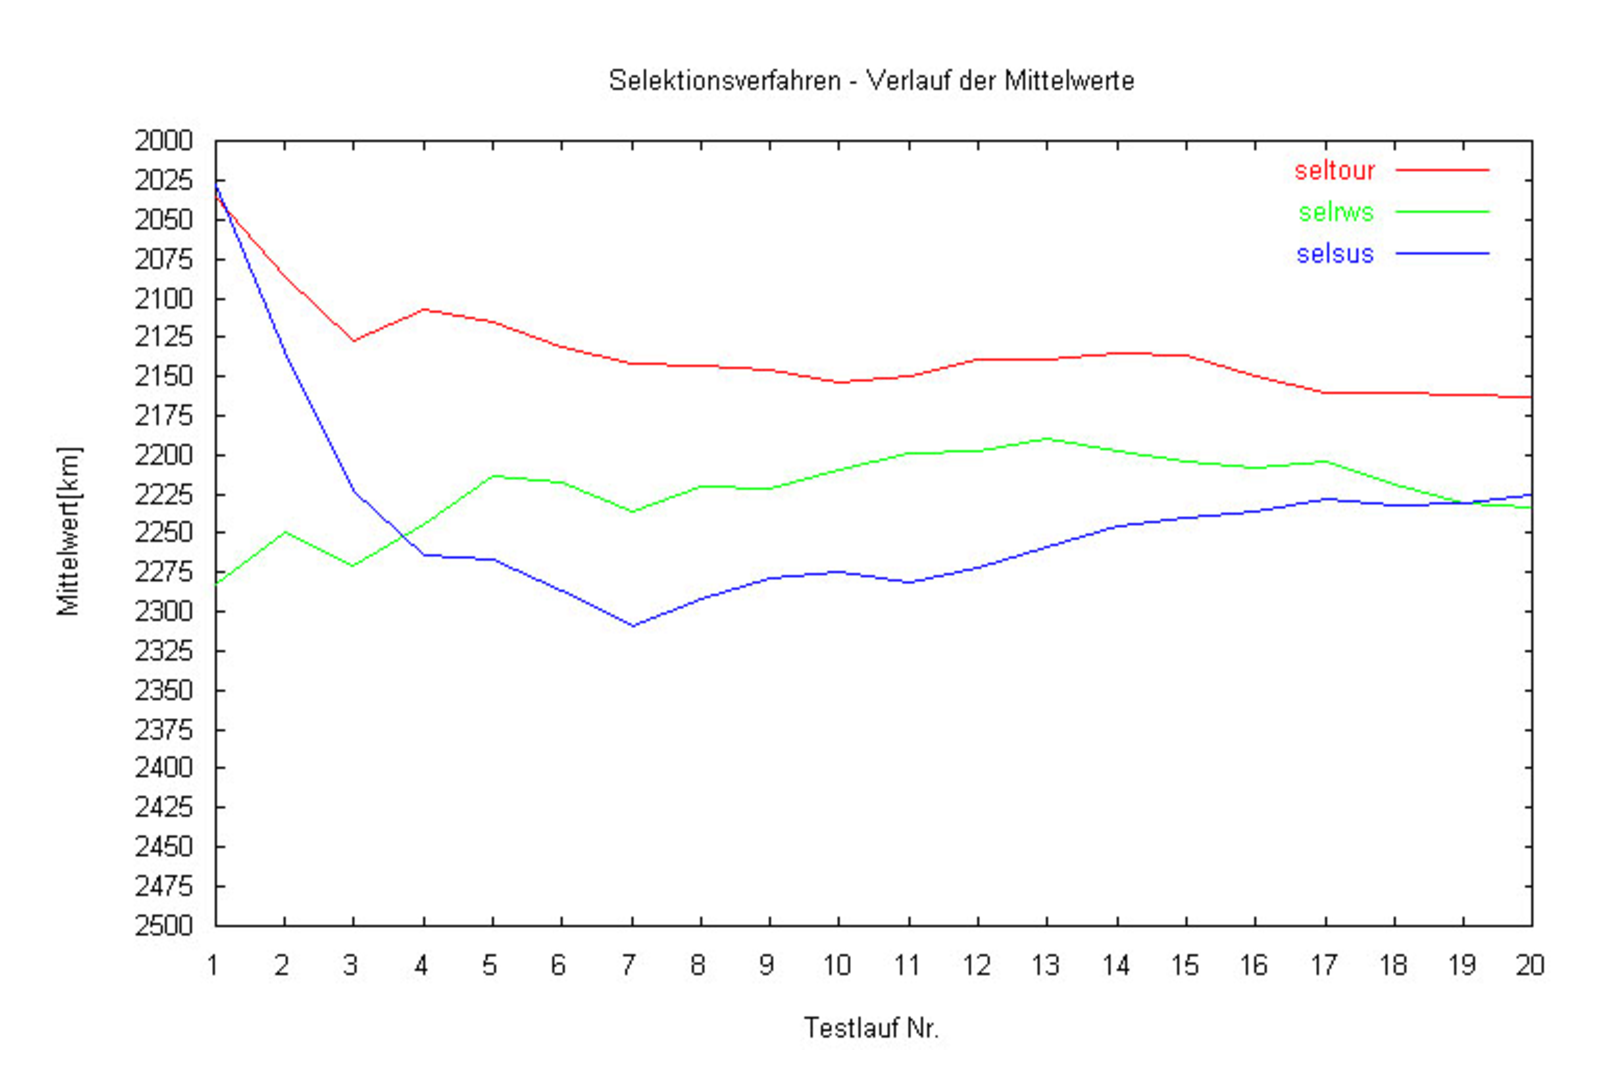
\includegraphics[width=1.0\textwidth]{../images/picMittelverlaufSelections}
  \caption{Verlauf der Mittelwerte der Selektionsarten 'selsus', 'selrws' und 'seltour'.}
  \label{fig:aufgabeDMittelwerte}
\end{figure}

Jedes der drei Verfahren zeigt eine Konvergenz der Mittelwerte gegen den Bereich 
$2150$ bis $2250$. Das 'selsus'-Verfahren erreicht früh seine besten Wert, fällt
dann aber steil ab und kovergiert die restlichen Läufe gegen den Konvergenzbereich.
Das Roulette-Wheel-Verfahren beginnt relativ schlecht und konvergiert schnell. Das
Tournament-Verfahren erreicht ebenfalls zu Beginn seinen besten Wert und konvergiert
auf etwas höherem Niveau als das 'selsus'-Verfahren gegen den Konvergenzbereich. 


\section{Aufgabe e}
\subsection{Rekombination}
Im Allgemeinen wird versucht aus den Genen der Eltern, mit Hilfe von
Rekombinationsmethoden neue Chromosomen bei den Nachfolgenerationen
zu erzeugen. Nach \cite{ErbenSkript} können so, mit neuen Chromosomen
auch neue Lösungen gefunden werden. Zuerst werden hierfür nach
\cite{ErbenSkript} die im Mating-Pool befindlichen Chromosome mit
einer vorbestimmten Wahrscheinlichkeit zur Paarung ausgewählt. 
'Unter den ausgewählten Chromosomen werden zufällige Elternpaare ( parents )
gebildet', \cite{ErbenSkript}. Danach werden je nach Rekombinationsart,
die zufällig ausgewählten Gene, unter den Eltern getauscht und auf die
Nachkommen übertragen.

\subsection{Rekombinationsoperator 'recpm'}
Bei herkömmlichen Rekombinationsverfahren, wie bspw. dem 'One-Point'- oder
auch 'Two-Point'-Crossover, kann es vorkommen, dass bestimmte Gene, innerhalb
eines Chromosoms doppelt vorkommen, was in bestimmten Problemstellungen
zu illegalen Lösungen führen würde. Gerade beim TSP-Problem, bei dem
jeder Ort nur einmal besucht werden darf, können derartige Lösungen
nicht akzeptiert werden. Das folgende Beispiel verdeutlicht das entstehen
einer illegalen Lösung für das TSP-Problem, anhand des 'Two-Point'-Crossovers.
Der dabei entstehende Nachkomme 'Kind1', trägt die Gene '1', '2' und '3' doppelt
in sich.

\begin{description}
  \item[Elter1-Chrom.:] 1 2 3 | 4 5 6 | 7 8
  \item[Elter2-Chrom.:] 4 6 7 | 3 1 2 | 5 8
  \item[Kind1-Chrom.:]  1 2 3   3 1 2   7 8 
\end{description}

Um derartigen Verdopplungen und illegalen Lösungen vorzubeugen, verwendet
man das Rekombinationsverfahren 'recpm', welches für 
'Partial Matching Recombination' steht. Die von Goldberg und Lingle 
vorgeschlagene Methode ist dabei besser bekannt als 'PMX', 
\cite{Berg93}. Dabei werden ebenfalls wieder die Rekombinationsbereiche
der beiden Elternchromosome ausgetauscht und den Kindern hinzugefügt.
Die restlichen Positionen der Kindchromosome werden mit den jeweils
eigenen Genen aufgefüllt, es sei denn, dass diese bereits in den 
rekombinierten Teilen auftauchen. Ist dies der Fall, so wird die 
Abbildungsfolge, die sich aus den Rekombinationsteilen ergibt, als
Mapping benutzt, um die übrigen Gene entsprechend zu tauschen und dem
Kind an entsprechender Stelle hinzuzufügen. Das Beispiel in Abb.
\ref{fig:RECPM1} und Abb. \ref{fig:RECPM2} soll die genannten Aspekte
verdeutlichen. 

\begin{figure} 
  \centering
  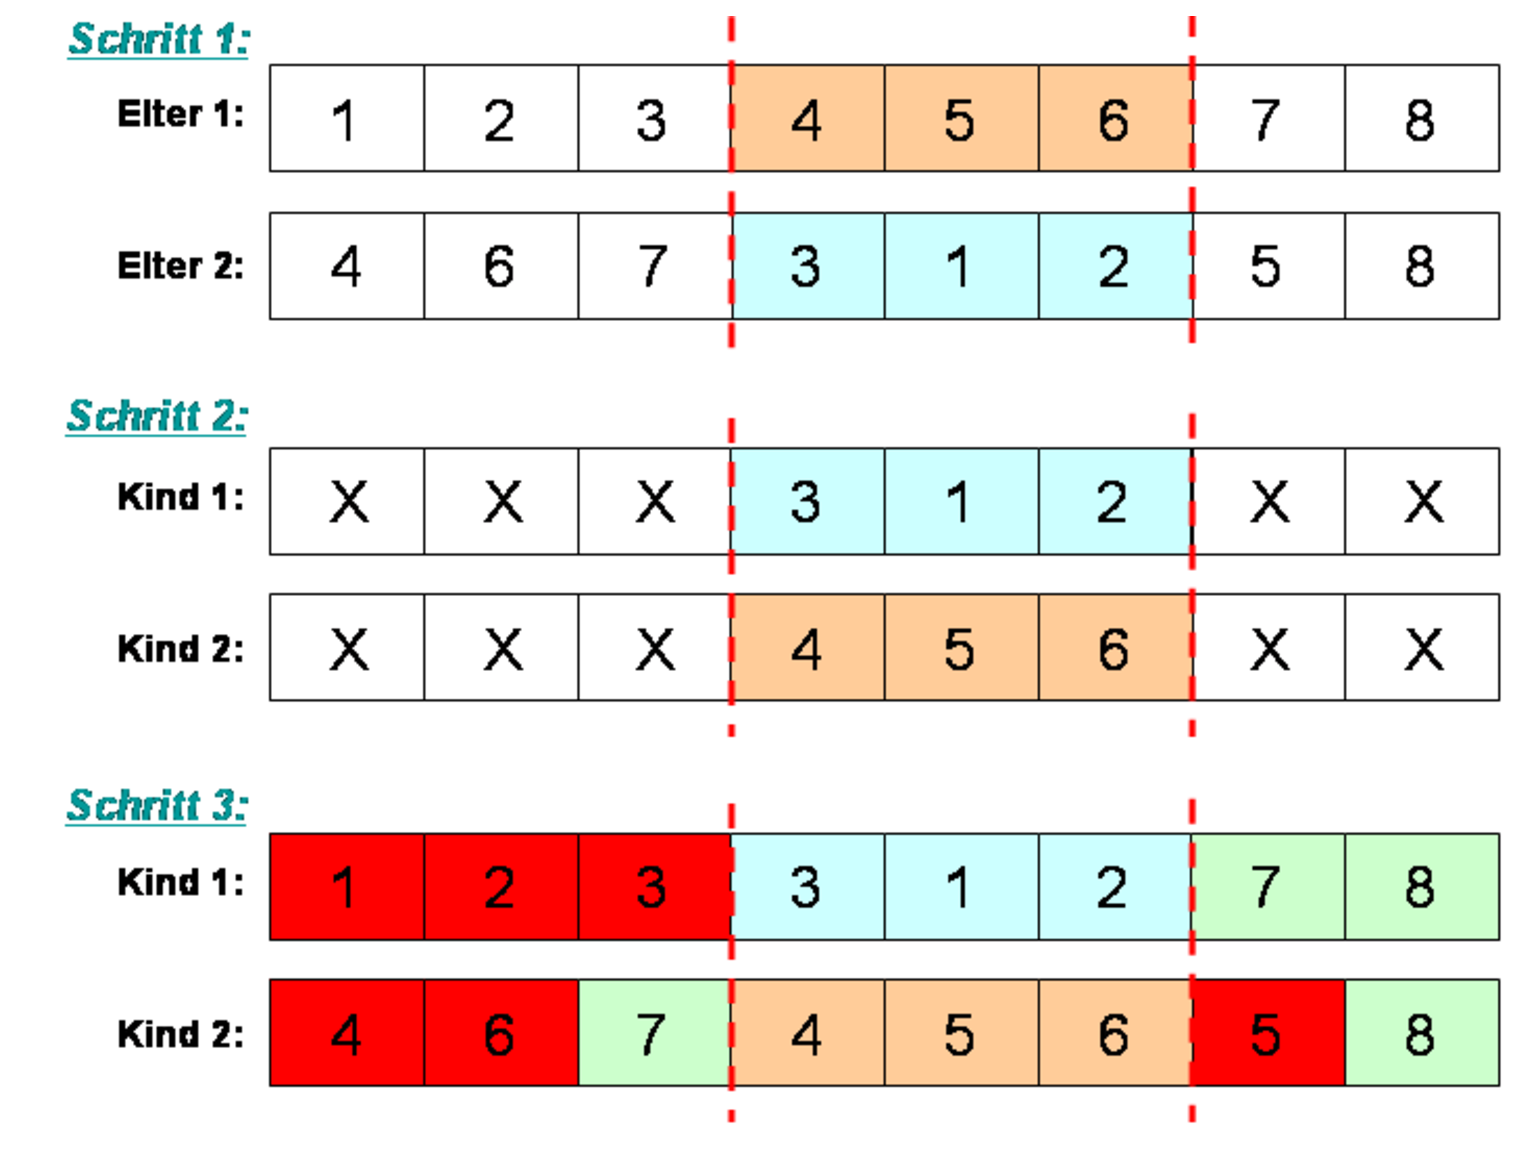
\includegraphics[width=0.8\textwidth]{../images/picRECPM1}
  \caption{Schritt 1-3 des 'Partial Recombination Crossover'}
  \label{fig:RECPM1}
\end{figure}

\begin{figure} 
  \centering
  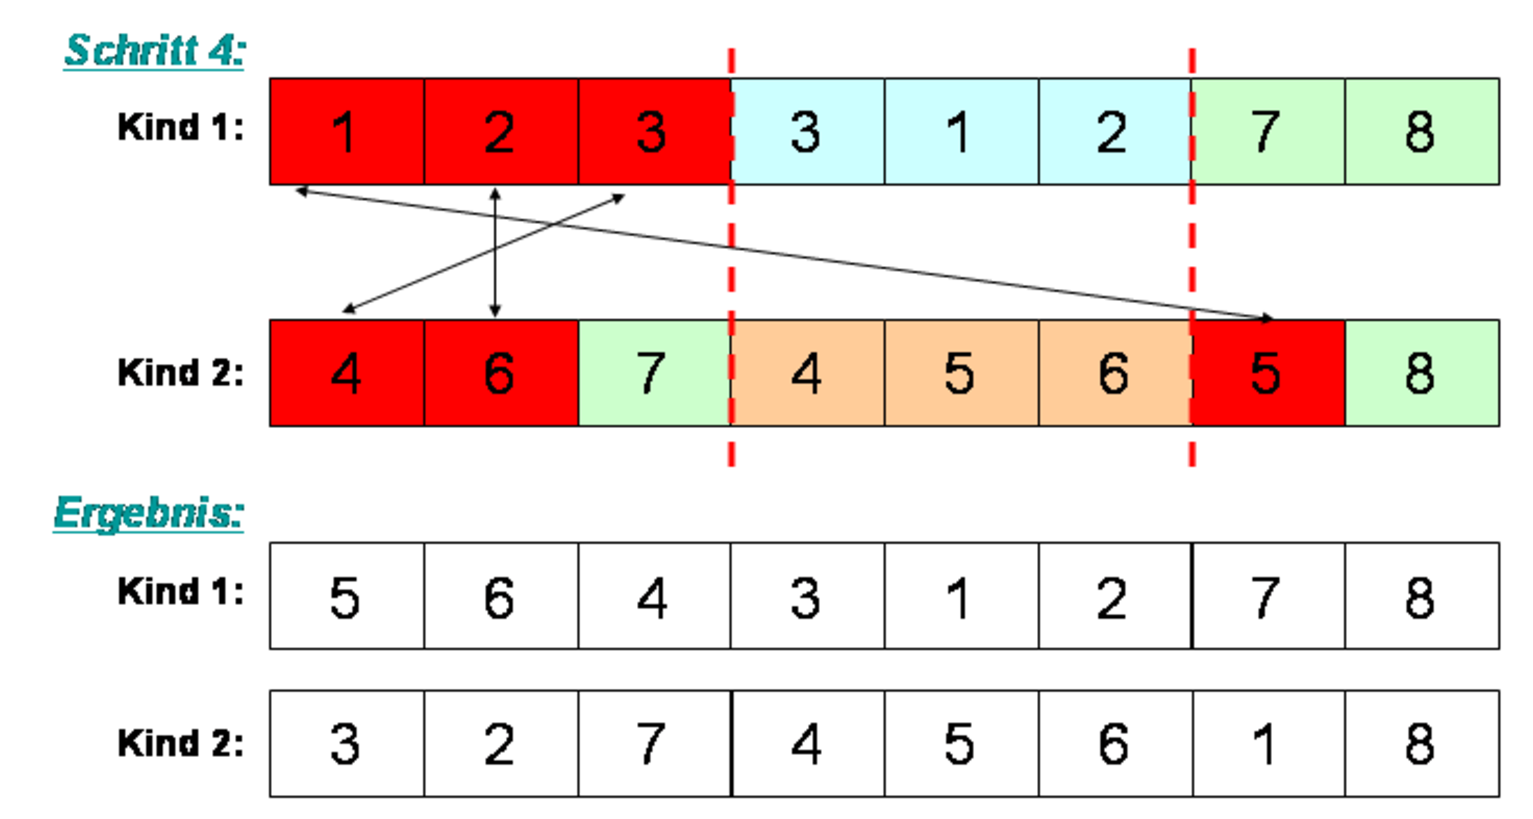
\includegraphics[width=0.8\textwidth]{../images/picRECPM2}
  \caption{Schritt 4 mit Ergebnis des 'PMX'}
  \label{fig:RECPM2}
\end{figure}

Im ersten Schritt wird der Rekombinationsbereich bestimmt. Die sich
darin befindlichen Gene werden im 2. Schritt zwischen den Eltern
ausgetauscht und den jeweiligen Kindern hinzugefügt. Die Gene
im Rekombinationsteil legen das später verwendete 'Mapping' fest
(hier 3<->4, 1<->5 und 2<->6). Im 3. Schritt
werden die Kindchromosome mit den jeweils restlichen Genen der Eltern
aufgefüllt. Die grün markierten Gene kennzeichnen dabei Werte, die
sich ohne Konflikte (Verdopplungen) hinzufügen lassen. Die rot Markierten
kennzeichnen die Gene, bei denen durch einfaches Hinzufügen ein illegaler
Zustand erreicht würde. Diese müssen über das erwähnte Mapping, gegeneinander
ausgetauscht werden. In diesem Fall wird bspw. die '1' von 'Kind1' gegen
die '5' von 'Kind2' ausgetauscht. Dieser Vorgang wiederholt sich solange, bis ein
legaler Zustand beider Chromosome erreicht ist.  

\subsection{Cycle Crossover}
Der \emph{Cycle Crossover}-Operator stellt sicher, dass die aus zwei gültigen
Elternchromosomen erzeugten Nachkommen wiederum gültige Individuen sind. Dazu
wird festgelegt, dass jedes Gen im Nachkommen von der selben Stelle eines der
Elternchromosome übernommen wird.

Der Algorithmus läuft in den folgenden Schritten ab, hier für die Erzeugung eines
Kindes $k$ aus zwei Eltern $e_1$ und $e_2$:

\begin{enumerate}
  \item Bestimmen einer zufälligen Startposition $s$.
  \item Übernehmen des Wertes an der Stelle $s$ an die selbe Stelle von $k$:
  $k[s] = e_1[s]$.
  \item Suchen der Position $i$ in $e_2$, an welcher der soeben gefundene Wert
  $e_1[s]$ steht.
  \item Übernehmen des Wertes aus $e_1$ nach $k$, welcher an der Stelle $i$
  steht: $k[i] = e_1[i]$.
\end{enumerate}

Dieser Vorgang wird solange wiederholt, bis sich ein Kreis (\emph{cycle})
gebildet hat, d.h. man zu einem bereits übernommenen Wert gelangt. Abschließend werden
die verbleibenden Stellen unverändert aus dem zweiten Elternteil übernommen.

\subsubsection{Implementierung in Matlab}
Listing \ref{lst:reccycle} zeigt unsere Implementierung des Cycle
Crossover-Operators in Matlab. Dabei haben wir die Struktur der Funktion
übernommen aus einer der GEATbx beiliegenden Operator-Funktionen, nämlich der
\texttt{recmp.m}.

\lstinputlisting[caption={Implementierung Cycle Crossover in Matlab},
label={lst:reccycle}]{../reccycle.m}

\subsection{Testläufe mit variierenden Rekombinations-Methoden}
Um die verschiedenen Rekombinationsoperatoren zu testen, wurden jeweils 20
Testläufe mit den folgenden Einstellungen vorgenommen:

\begin{description}
  \item[Anzahl Subpopulationen:] 12
  \item[Anzahl Individuen:] 60
  \item[Selektionsoperator:] Tournament-Selektion, \texttt{seltour}
  \item[Mutationsoperator:] Kombination aus \texttt{mutswap}, \texttt{mutmove} 
	und \texttt{mutinvert}
  \item[Rekombinationsoperator:] Variation zwischen \texttt{recgp},
  \texttt{recpm} und dem eigenimplementierten \texttt{reccycle}
\end{description}

Tabelle \ref{tbl:aufgabeE-ergebnisse} zeigt die Ergebnisse der Testläufe. 

\begin{table}
	\sffamily
	\centering
	\footnotesize
	\begin{tabularx}{\textwidth}{TlllllX}
		\toprule
		\multicolumn{1}{@{}N}{Rekombination} &
		\multicolumn{1}{V{5em}@{}}{Mittelwert $\bar{x}$} &
		\multicolumn{1}{V{6.5em}@{}}{Standardabw. $\sigma_x$} &
		\multicolumn{1}{V{9em}@{}}{Minimalwert in Lauf $r$, Generation $g$} &
		\multicolumn{1}{V{9em}@{}}{Maximalwert in Lauf $r$, Generation $g$} & 
		\multicolumn{1}{V{5em}@{}}{Mittelwert CPU-Zeit [s]} \\
		\midrule\addlinespace
		recgp & 2201,50 & 106,00 & 2035, $r = 11$, $g = 100$ & 2353, $r = 1$, $g
		= 100$ & 131,31\\
		\midrule
		recpm & \textbf{2195,45} & 97,81 & \textbf{2034}, $r = 1$, $g = 82$ & 2358, $r = 19$, $g = 98$ & 31,95\\
		\midrule
		reccycle & 2302,30 & \textbf{89,05} & 2147, $r = 6$, $g = 96$ & 2449, $r = 3$, $g = 98$ & 19,65\\

		\addlinespace\bottomrule
		\end{tabularx}
	\caption{Zusammengefasste Ergebnisse der Testreihe}
	\label{tbl:aufgabeE-ergebnisse}
\end{table}
 
\subsubsection{Interpretation der Ergebnisse}
Wie man an den Ergebnissen der Testreihe ablesen kann, scheint es zwischen den
einzelnen Rekombinationsoperatoren keine signifikanten Unterschiede zu geben. Das
beste Mittelwertergebnis dieser Testreihe mit ca. 2195 km wurde unter Verwendung
des \texttt{recpm}-Verfahrens erreicht. Der von uns implementierte
\texttt{reccycle}-Operator schnitt bei den Mittelwerten schlechter ab, jedoch
erzielte er die geringsten Standardabweichung in der Testreihe. Was man
allerdings festhalten muss, ist die Tatsache, dass \texttt{recgp} einen erheblich
höheren CPU-Aufwand erfordert als der \texttt{reccycle}-Operator. Hier sind
benötigte Ergebnis-Güte und Rechenzeit gegeneinander abzuwägen. Abbildung
\ref{fig:aufgabeE-plot} zeigt nochmals den kompletten Verlauf der Testergebnisse
in graphischer Form.

\begin{figure}
  \centering
  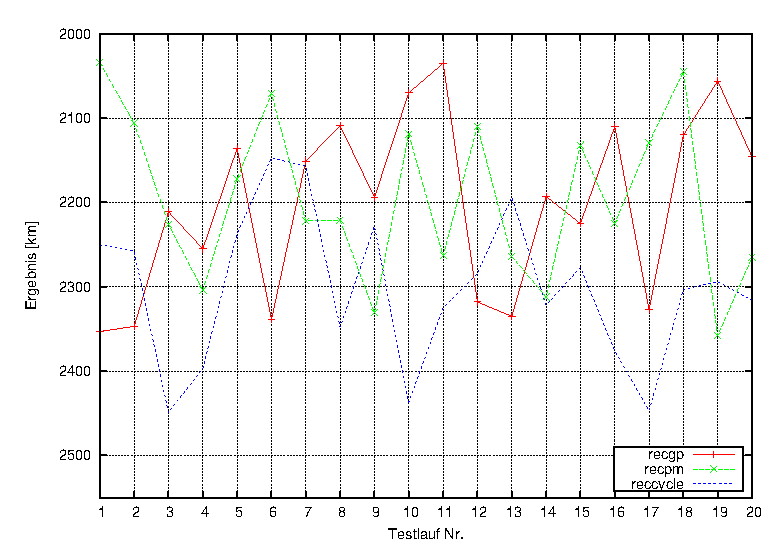
\includegraphics[width=1.0\textwidth]{../images/aufgabeE-plot}
  \caption{Grafische Darstellung der Testreihe mit verschiedenen Rekombinationsoperatoren}
  \label{fig:aufgabeE-plot}
\end{figure}

\section{Aufgabe f}
\subsection{Mutation}
\label{subsec:Mutation}
Im Allgemeinen wird versucht mit Hilfe von Mutationsmechanismen aus einem
bestehenden Individuum, ein Individuum mit neuen Eigenschaften zu erzeugen.
Dies geschieht nach \cite{ErbenSkript} indem aus dem Genpool aller Individuen,
zufällig ein Gen ausgwählt wird, das über einen bestimmten Mutations-Algorithmus
verändert wird. Über Mutation wird oft versucht neue Lösungen zu erzeugen, welche
alleine durch die Regeln der Selektion und Rekombination oft nicht erreicht werden
könnten. So wird nach \cite{url:UniPaderborn} durch Mutation 'eine
frühzeitige Konvergenz eines Algorithmus verhindert'. Im Folgenden werden hierzu
die unterschiedlichen Mutationsoperatoren 'mutswap ', 'mutmove' und  'mutinvert'
genauer betrachtet.

\subsection{Mutationsoperator 'mutswap'}
\label{subsec:mutswap}
Die Mutationsart 'mutswap' ist ein einfacher Algortihmus, bei dem nach 
\cite{url:geatbx-documentation} 'eine zufällig ausgwählte Variable eines
Indivduums, mit einer anderen Variable des selben Individuums vertauscht
wird'. Unter einer Variablen ist ein bestimmtes Gen eines Chromosoms zu
verstehen. Die folgende Abbildung \ref{fig:MUTSWAP} veranschaulicht dies.
Hierbei werden die Positionen der Variabeln mit den Werten $7$ und $3$
vertauscht.

\begin{figure} 
  \centering
  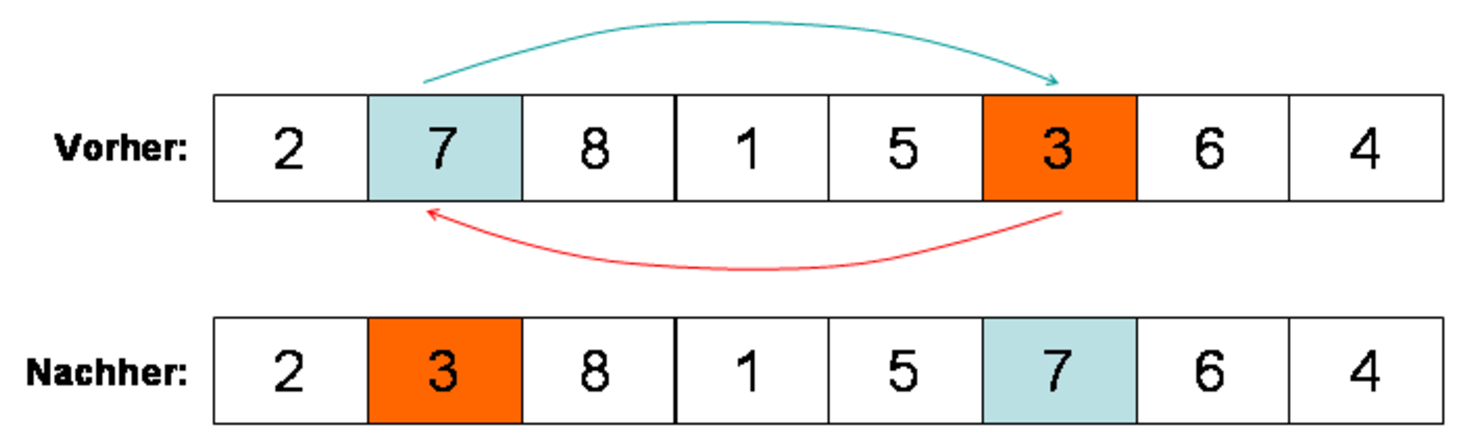
\includegraphics[width=0.7\textwidth]{../images/picMUTSWAP}
  \caption{Mutation mit 'mutswap'-Operator}
  \label{fig:MUTSWAP}
\end{figure}

\subsection{Mutationsoperator 'mutmove'}
\label{subsec:mutmove}
Bei der 'mutmove'-Methode handelt es sich um eine Mutation, bei der 
die Position \textit{i} einer Variabeln  innerhalb eines Chromosoms
an eine neue Position \textit{k} verschoben wird. Alle Variabeln
mit Positionen ab \textit{i+1} bis \textit{k} rutschen während
der Verschiebung um eine Position nach vorne.  
Abbildung \ref{fig:MUTMOVE} verdeutlicht dies. Hierbei wird
die Variable mit dem Wert $7$ um vier Positionen nach rechts verschoben.
Dabei rutschen die Variabeln mit den Werten $8$, $1$, $5$ und $3$ um je
eine Position nach vorne.

\begin{figure} 
  \centering
  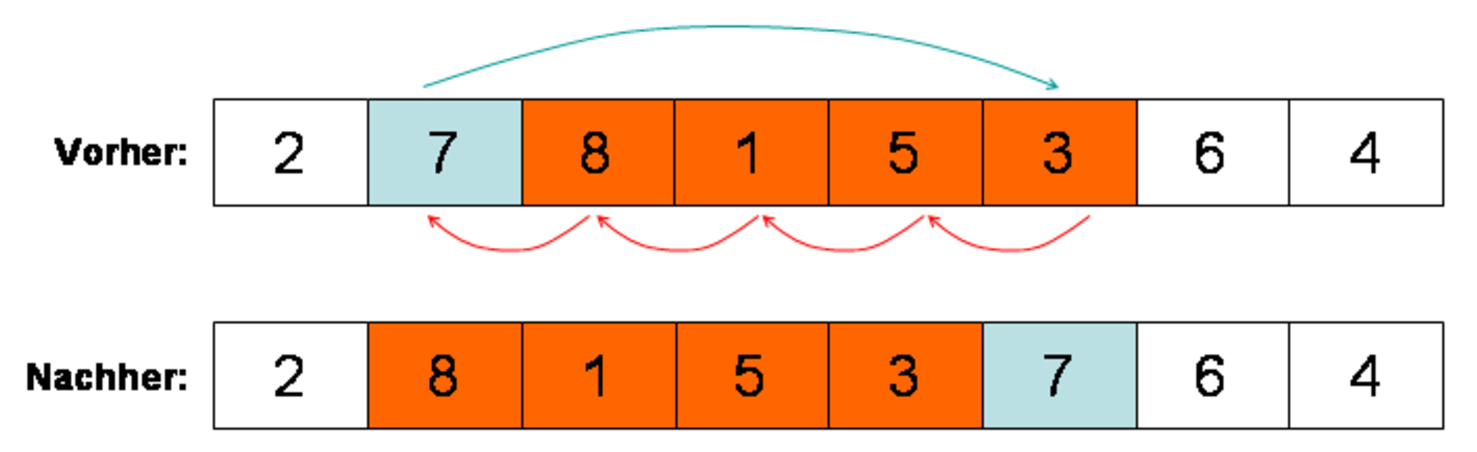
\includegraphics[width=0.7\textwidth]{../images/picMUTMOVE}
  \caption{Mutation mit 'mutmove'-Operator}
  \label{fig:MUTMOVE}
\end{figure}

\subsection{Mutationsoperator 'mutinvert'}
\label{subsec:mutinvert}
Bei Verwendung des 'mutinvert'-Operators wird nach
\cite{url:geatbx-documentation} 'jede Variablen-Position innerhalb
zweier Positionen invertiert'. D. h. es wird zuerst die Sequenz
oder Gruppe von Variabeln ermittelt, die zwischen zwei zufälligen
Positionen liegen. Die Positionen dieser Sequenz-Gruppe werden
anschließend invertiert. Abbildung \ref{fig:MUTINVERT} zeigt wie
aus der Sequenz $8$, $1$, $5$, $3$, die Sequenz $3$, $5$, $1$, $8$
entsteht.   

\begin{figure} 
  \centering
  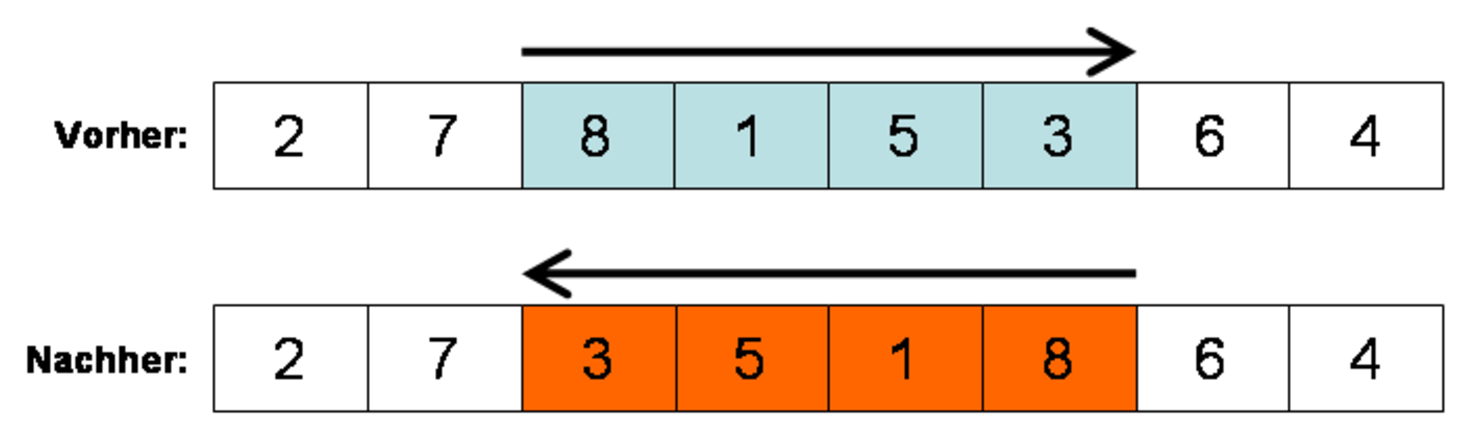
\includegraphics[width=0.7\textwidth]{../images/picMUTINVERT}
  \caption{Mutation mit 'mutinvert'-Operator}
  \label{fig:MUTINVERT}
\end{figure}

\subsection{Einsatz aller Mutationsoperatoren}
\label{subsec:AlleMutationen}
Wie am Anfang des Kapitels \ref{subsec:Mutation} beschrieben, ist das
Ziel bei der Mutation, neue Eigenschaften bei Individuen zu erzeugen.
Würde man nun 1 Mutationsart einsetzen, so könnte es vorkommen, dass
ein bereits ein oder mehrfach mutiertes Individuum, wieder in seinen
Ausgangszustand vor der ersten Mutation versetzt wird. Des Weiteren
könnte es vorkommen, dass eine bereits bestehende Veränderung im Erbgut der
Nackommen ebenfalls wieder zurückmutiert werden würde. D.h. man
würde durch erneutes Anwenden quasi alle Mutationsschritte rückgängig machen.
So wäre es möglich, dass bei 'mutswap' exakt die gleichen Variabeln
zurückgetauscht werden würden. Achtmaliges Anwenden der Operation 
'mutmove', würde eine Variable bspw. wieder an ihre
Ausgangsposition zurückversetzen. Auch bei 'mutinvert' wäre es möglich,
dass eine bereits invertierte Sequenz zurück invertiert wird.

Abbildung \ref{fig:MUTINVERTBackchange} illustriert am Beispiel von 'mutswap'
das unerwünschte Ergebnis nach mehrfachen Anwenden derselben Mutation.

Aus diesem Grund mischt man die angesprochenen Mutationsverfahren innerhalb
eines Testlaufs. Dadurch minimiert sich die Wahrscheinlichkeit, mit derselben
Mutationsart, eine bereits erreichte und gewünschte Veränderung des
Erbgutes wieder versehentlich rückgängig zu machen.
 
\begin{figure} 
  \centering
  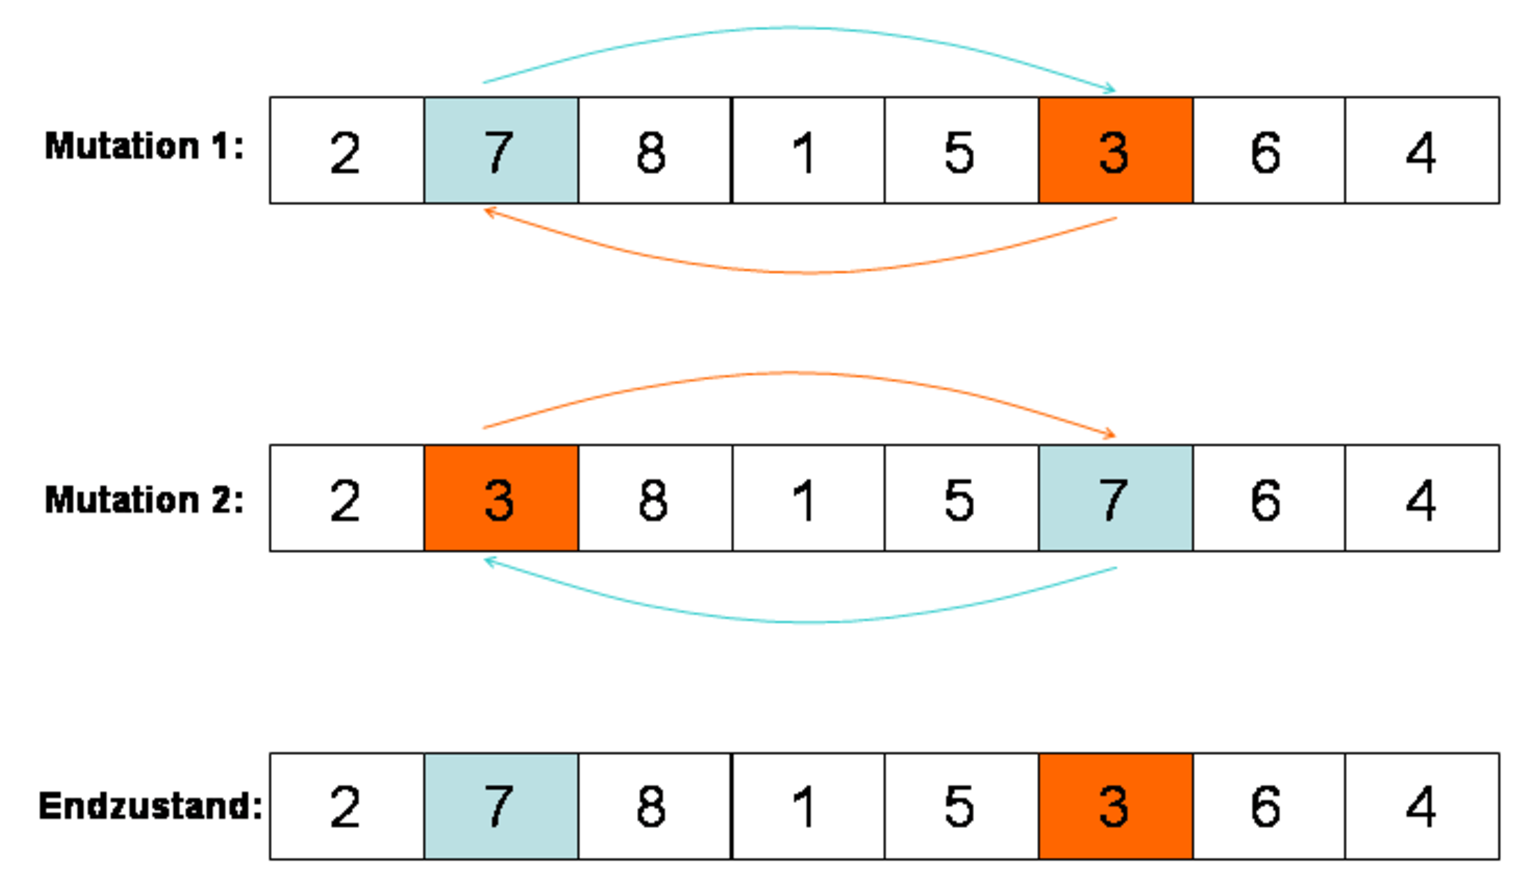
\includegraphics[width=0.6\textwidth]{../images/picMUTINVERTBackchange}
  \caption{Unerwünschter Zustand nach zweimaligen Anwenden von 'mutswap'.}
  \label{fig:MUTINVERTBackchange}
\end{figure}

\subsection{Testläufe mit variierenden Mutationsraten}
\label{subsec:TestlaufeMuationsraten}
Für die Durchführung der Testreihen in Aufgabe f), wurde eine 
angepasste Version des \ref{subsec:ArchitekturTestsystem} beschriebenen
Testskriptes benutzt.

\begin{description}
  \item[Mutations-Verfahren:] 'mutswap', 'mutmove', 'mutinvert' (kombiniert)
  \item[Mut.-Raten:] 0.001, 0.005, 0.01, 0.05, 0.08, 0.1, 0.2, 0.3, 0.4, 0.5, 1, 3, 5, 10, 15, 20, 25
\end{description} 

Es wurden 16 Testreihen, mit jeweils 20 Testläufen durchgeführt. Jeder der
Testläufe wurde mit einer Kombination der drei Muationsarten durchgeführt.
Zwischen den einzelnen Testläufen wurde die Muationsrate variiert.
Die Ergebnisse aller Testläufe werden hierzu in Tabelle
\ref{tbl:aufgabeF-ergebnisse} dargestellt.

\begin{table}
	\sffamily
	\centering
	\footnotesize
	\begin{tabularx}{\textwidth}{NXlllll}
		\toprule
		\multicolumn{1}{@{}N}{Mut.-Rate} &
		\multicolumn{1}{V{3.5em}@{}}{Subpop.} &
		\multicolumn{1}{V{3.5em}@{}}{Indiv.} &
		\multicolumn{1}{V{5em}@{}}{Mittelwert $\bar{x}$} &
		\multicolumn{1}{V{6.5em}@{}}{Standardabw. $\sigma_x$} &
		\multicolumn{1}{V{9em}@{}}{Minimalwert in Lauf $r$, Generation $g$} &
		\multicolumn{1}{V{9em}@{}}{Maximalwert in Lauf $r$, Generation $g$} \\
		\midrule\addlinespace
		
		0.001 & 12 & 60 & 2387.95 & 110.29 & 2217 , $r = 8$, $g = 100$ & 2611 , $r = 18$, $g = 92$ \\ \cmidrule(lr){1-7}
		0.005 & 12 & 60 & 2170.20 & 80.31 & 2062 , $r = 11$, $g = 97$ & 2422 , $r = 16$, $g = 94$ \\ \cmidrule(lr){1-7}
		0.01 & 12 & 60 & \textbf{2138.45} & \textbf{58.19} & 2059 , $r = 7$, $g = 87$ & \textbf{2249} , $r = 4$, $g = 99$ \\ \cmidrule(lr){1-7}
		0.05 & 12 & 60 & 2223.45 & 101.40 & 2084 , $r = 1$, $g = 97$ & 2423 , $r = 18$, $g = 94$ \\ \cmidrule(lr){1-7}
		0.08 & 12 & 60 & 2379.30 & 156.63 & 2121 , $r = 16$, $g = 96$ & 2633 , $r = 14$, $g = 88$ \\ \cmidrule(lr){1-7}
		0.1 & 12 & 60 & 2456.35 & 124.13 & 2257 , $r = 16$, $g = 95$ & 2742 , $r = 7$, $g = 83$ \\ \cmidrule(lr){1-7}
		0.2 & 12 & 60 & 2772.90 & 136.93 & 2613 , $r = 8$, $g = 99$ & 3072 , $r = 14$, $g = 74$ \\ \cmidrule(lr){1-7}
		0.3 & 12 & 60 & 3029.95 & 131.85 & 2834 , $r = 15$, $g = 84$ & 3372 , $r = 2$, $g = 72$ \\ \cmidrule(lr){1-7}
		0.4 & 12 & 60 & 2159.30 & 69.12 & 2047 , $r = 11$, $g = 100$ & 2278 , $r = 13$, $g = 100$ \\ \cmidrule(lr){1-7}
		0.5 & 12 & 60 & 2171.20 & 93.45 & \textbf{2026} , $r = 8$, $g = 92$ & 2339 , $r = 16$, $g = 93$ \\ \cmidrule(lr){1-7}		
		1 & 12 & 60 & 2217.30 & 89.41 & 2065 , $r = 3$, $g = 86$ & 2403 , $r = 2$, $g = 95$ \\ \cmidrule(lr){1-7}
		3 & 12 & 60 & 2449.45 & 110.05 & 2229 , $r = 13$, $g = 100$ & 2606 , $r = 2$, $g = 90$ \\ \cmidrule(lr){1-7}
 	 	5 & 12 & 60 & 2677.10 & 138.78 & 2424 , $r = 1$, $g = 93$ & 2898 , $r = 20$, $g = 72$ \\ \cmidrule(lr){1-7}
		10 & 12 & 60 & 3061.95 & 172.52 & 2769 , $r = 13$, $g = 92$ & 3334 , $r = 12$, $g = 90$ \\ \cmidrule(lr){1-7}
		15 & 12 & 60 & 3287.40 & 161.55 & 2997 , $r = 17$, $g = 100$ & 3582 , $r = 13$, $g = 95$ \\ \cmidrule(lr){1-7}
		20 & 12 & 60 & 3395.55 & 110.47 & 3151 , $r = 20$, $g = 53$ & 3600 , $r = 5$, $g = 95$ \\ 
								
		\addlinespace\bottomrule
		\end{tabularx}
	\caption{Ergebnisse aus 16 Testreihen a 20 Testläufe, mit kombinierten Mutationsverfahren und unterschiedlichen Mutationsraten.}
	\label{tbl:aufgabeF-ergebnisse}
\end{table}

\subsubsection{Interpretation der Ergebnisse}
Tendenziell zeigt sich durch eine Erhöhung der Mutationsrate eine eher negative
Auswirkung auf die einzelnen Testergebnisse. So führen die hohen Mutationsraten
ab '1', zu einer deutlichen Verschlechterung der Werte. Auch die Ergebnisse zwischen
den Raten '0.1' und '0.3', verschlechtern sich zusehens mit der Erhöhung.
Die besten Ergebnisse konnten mit Mutationsraten zwischen '0.005' bis '0.05',
sowie '0.4' bis '1' erzielt werden. Der minimalste Wert von 2026 Kilometern, 
wurde dabei mit der Mutationsrate von '0.5' erreicht. Das durschnittlich
beste Ergebnis wurde mit der Mutationsrate von '0.01' und einem Mittelwert von
2138.45 erzielt. Die Standardabweichung von 58.19, weist dabei ebenfalls den 
niedrigsten Wert aller Testläufe auf. 


\section{Aufgabe g}
\subsection{Optimale Parameter}
Durch die in dieser Arbeit durchgeführten Testläufe ergeben sich für uns die
optimalen Parameter wie folgt:

\begin{description}
  \item[Anzahl Generationen:] 100
  \item[Anzahl Subpopulationen:] 12
  \item[Anzahl Individuen:] 60
  \item[Selektionsoperator:] Tournament Selection, \texttt{seltour}
  \item[Rekombinationsoperator:] Recombination Partial Matching, \texttt{recpm}
  \item[Mutationsoperator:] Kombination aus \texttt{mutswap}, \texttt{mutmove} 
	und \texttt{mutinvert}
\end{description}

\subsection{Testläufe mit variierenden TSP-Problemen}
Abschließend führen wir jeweils 20 Testläufe mit den o.g. Parametern und drei
verschiedenen TSP-Problemen durch; die Ergebnisse sind in Tabelle
\ref{tbl:aufgabeG-ergebnisse} aufgezeigt.

\begin{table}
	\sffamily
	\centering
	\footnotesize
	
	\begin{threeparttable}
	\begin{tabularx}{\textwidth}{TXlllp{7em}p{7em}}
		\toprule
		\multicolumn{1}{@{}N}{TSP-Bsp.} &
		\multicolumn{1}{V{3em}@{}}{Subpop.} &
		\multicolumn{1}{V{3em}@{}}{Indiv.} &
		\multicolumn{1}{V{5em}@{}}{Mittelwert $\bar{x}$} &
		\multicolumn{1}{V{6.5em}@{}}{Standardabw. $\sigma_x$} &
		\multicolumn{1}{V{8em}@{}}{Minimalwert in Lauf $r$, Generation $g$} &
		\multicolumn{1}{V{8em}@{}}{Maximalwert in Lauf $r$, Generation $g$} \\
		\midrule\addlinespace
		bays29 & 12 & 60 & 2140,65 & 87,39 & 2028, $r = 13$, $g = 96$ & 2375, $r = 6$, $g = 95$ \\
		\midrule
		bayg29 & 12 & 60 & 1692,90 & 39,54 & 1610, $r = 16$, $g = 89$ & 1746, $r = 13$, $g = 97$ \\
		\midrule
		berlin52 & 12 & 60 & 11218,55 & 660,23 & 9854, $r = 20$, $g = 100$ & 12326, $r = 2$, $g = 99$ \\ \cmidrule(rl){1-7}
		berlin52\tnote{1} & 12 & 60 & 8262,10& 278,77 & 7786, $r = 18$, $g = 362$ & 8931, $r = 7$, $g = 394$ \\ \cmidrule(rl){1-7}
		berlin52\tnote{1} & 20 & 100 & \textbf{8110,45} & \textbf{193,89} & \textbf{7734}, $r = 1$, $g = 336$ & 8424, $r = 8$, $g = 330$ \\

		\addlinespace\bottomrule
	\end{tabularx}
	\begin{tablenotes}
	  \footnotesize\normalfont
    	\item [1] Anzahl der Generationen: 400
 	\end{tablenotes}
	\end{threeparttable}
	\caption{Ergebnisse der Testreihe}
	\label{tbl:aufgabeG-ergebnisse}
\end{table}

\subsubsection{Interpretation der Ergebnisse}
Der erreichte Wert für \texttt{bays29} erschien uns mit 2028 nahe genug am
Idealwert 2020. Für \texttt{bayg29} konnte sogar der bestbekannte Wert von 1610
(vgl. \cite[Appendix]{Reinelt94}) erreicht werden.
Für diese beiden TSP-Beispiele scheinen unsere gefunden Einstellungen demnach
sehr gut zu funktionieren. Im Gegensatz dazu verfehlten wir bei dem Problem mit
52 Knoten den Optimalwert 7542 um Längen. Daher versuchten wir, durch
Heraufsetzen der Generationen hier noch Verbesserungen zu erlangen, was uns in
Maßen auch gelang. Durch Einsatz von 400 Generationen wurden die Ergebnisse
deutlich verbessert, wie die Tabelle zeigt. 

Durch die Erhöhung der Subpopulationen sowie der Anzahl der Individuen im letzten
Testlauf konnten weitere leichte Verbesserungen erreicht werden. So ergibt sich
der von uns erreichte Minimalwert zu 7734.



%%%
%%% Anhaenge: Glossar, Bibliographie...
%%%

\cleardoublepage % oder \clearpage
\phantomsection

% Anhang
\appendix
\pdfbookmark[-1]{\appendixname}{\appendixname} 

% Quellcode des Test-Skripts einbinden
\chapter{Quellcode Testskript}
\lstinputlisting{../tsp.m}

%%% Bibliographie-Stil
% abbrvdin, alphadin, plaindin, unsrtdin
\bibliographystyle{alphadin}

%%% Anstatt 'Literatur' -> 'Quellen'
\renewcommand{\bibname}{Quellen}

%%% Bibliographie ausgeben
\bibliography{Quellen}

\end{document}